\documentclass[12pt]{article}
\usepackage[utf8]{inputenc}
\usepackage[T1]{fontenc}
\usepackage[a4paper, margin=1in]{geometry}
\usepackage{xcolor}
\usepackage{titlesec}
\usepackage{lmodern}
\usepackage{amsmath, amssymb}
\usepackage{enumitem}
\usepackage{graphicx}
\usepackage{pdfpages}
\usepackage{fancyhdr}
\usepackage{float}
\usepackage{hyperref}

% Colors for sections
\definecolor{chaptercolor}{RGB}{0, 51, 102} 
\definecolor{sectioncolor}{RGB}{0, 102, 102}   
\definecolor{subsectioncolor}{RGB}{60, 60, 60} 

% Section formatting
\titleformat{\section}
  {\normalfont\Large\bfseries\color{chaptercolor}}{\thesection}{1em}{}
\titlespacing*{\section}{0pt}{20pt}{10pt}
\titleformat{\subsection}
  {\normalfont\large\bfseries\color{sectioncolor}}{\thesubsection}{1em}{}
\titlespacing*{\subsection}{0pt}{15pt}{8pt}
\titleformat{\subsubsection}
  {\normalfont\normalsize\bfseries\color{subsectioncolor}}{\thesubsubsection}{1em}{}
\titlespacing*{\subsubsection}{0pt}{12pt}{6pt}

\title{\textbf{Hubble Constant with the Pantheon+SH0ES Supernova Sample}}
\author{Pranauv C.H}
\date{}

% Fancyhdr setup
\setlength{\headheight}{15pt}
\pagestyle{fancy}
\fancyhf{}
\fancyhead[R]{Hubble Constant with the Pantheon+SH0ES Supernova Sample}
\fancyfoot[C]{\thepage}

\begin{document}

\maketitle


\begin{abstract}
We present a cosmological analysis of the Pantheon+SH0ES Type Ia supernova dataset within the flat $\Lambda$CDM framework. 
Using numerical integration of the luminosity distance and $\chi^2$ minimization, we obtain best-fit parameters of
\[
H_0 = 72.97 \pm 0.26 \ \mathrm{km\,s^{-1}\,Mpc^{-1}}, \quad \Omega_m = 0.351 \pm 0.019.
\]
These values are consistent with local Cepheid-calibrated measurements from the SH0ES program but remain in significant 
tension with the Planck 2018 cosmic microwave background determination of $H_0 = 67.4 \pm 0.5\ \mathrm{km\,s^{-1}\,Mpc^{-1}}$. 
The resulting age of the Universe is estimated as $t_0 \approx 12.36$ Gyr, notably lower than the 13.8 Gyr inferred from 
CMB-based $\Lambda$CDM cosmology. Subsample tests (low-$z$ vs.\ high-$z$ supernovae) and fixed-parameter fits demonstrate 
the robustness of the results across redshift ranges and cosmological priors. These findings reinforce the persistence of 
the Hubble tension and highlight either residual systematics or physics beyond the standard model.
\end{abstract}

\newpage
\tableofcontents

\newpage
\section{Introduction}

The discovery of the relation between galaxy redshifts and their distances by Edwin Hubble in 1929 established the expanding–Universe 
paradigm and laid the foundation for modern observational cosmology. Subsequent decades have been dedicated to refining the measurement of 
the Hubble constant ($H_0$), which quantifies the present–day expansion rate of the Universe.

Type Ia supernovae (SNe~Ia) have become essential probes in this effort. Their remarkable uniformity in peak luminosities, combined with 
empirical corrections, makes them powerful standardizable candles for measuring extragalactic distances. Large–scale compilations such as 
the Pantheon+ sample have provided unprecedented statistical precision, enabling cosmological analyses that rival those of other probes. 
The Pantheon+SH0ES dataset, in particular, combines high–redshift supernovae with nearby Cepheid–calibrated SNe~Ia to anchor the cosmic distance ladder.

In the framework of the $\Lambda$CDM model, the Universe is described as spatially flat, dominated by cold dark matter ($\Omega_m$) and a 
cosmological constant ($\Omega_\Lambda$). Within this model, the Hubble parameter evolves with redshift according to the Friedmann equation, 
allowing theoretical predictions of distance measures that can be directly compared with supernova observations.

A key focus of contemporary cosmology is the so–called ``Hubble tension''—the discrepancy between early–Universe inferences of $H_0$ from 
cosmic microwave background measurements (Planck 2018) and late–Universe direct determinations from Cepheid–calibrated SNe~Ia (SH0ES). 
While Planck data favors a value near $67.4 \,\mathrm{km\,s^{-1}\,Mpc^{-1}}$, SH0ES measurements indicate a significantly higher value 
around $73 \,\mathrm{km\,s^{-1}\,Mpc^{-1}}$. Resolving this discrepancy remains one of the most pressing challenges in cosmology.

The objective of this study is to analyze the Pantheon+SH0ES dataset under the flat $\Lambda$CDM framework. By fitting theoretical 
distance moduli to observed supernova data, we aim to obtain best–fit values of $H_0$ and $\Omega_m$, estimate the corresponding age of 
the Universe, and assess the results in the context of the Hubble tension.

\section{Data Selection \& Preprocessing}
\subsection{Data Source}
The data used in this study are drawn from the Pantheon+SH0ES compilation of Type Ia supernovae, one of the most comprehensive SN~Ia datasets currently available. 
It includes more than 1{,}500 supernovae across a redshift range extending from the nearby Universe ($z \sim 0.01$) to high redshift ($z \sim 2.3$). 
The SH0ES component provides an absolute calibration through Cepheid–variable distance measurements in nearby galaxies hosting SNe~Ia. 
The dataset contains observed redshifts, measured distance moduli, and associated uncertainties, which together provide the basis for cosmological parameter estimation.

\subsection{Data Cleaning and Preparation}
The raw dataset was inspected for missing or invalid entries, and non–physical values were excluded from further analysis. Each supernova entry provides a redshift $z$, 
an observed distance modulus $\mu_{\mathrm{obs}}$, and an uncertainty $\sigma_\mu$. To ensure reliability, only supernovae with well–defined uncertainties were retained. 
The resulting dataset forms a robust basis for $\chi^2$ minimization against theoretical cosmological predictions.

\subsection{Dataset Overview}
The Pantheon+SH0ES sample spans a wide redshift range, enabling both low–redshift calibration and high–redshift cosmological testing. The inclusion of SH0ES calibration 
ensures sensitivity to the present–day expansion rate ($H_0$), while the broad redshift coverage constrains the evolution of the Hubble parameter through the matter 
density parameter ($\Omega_m$).


\begin{figure}[H]
    \centering
    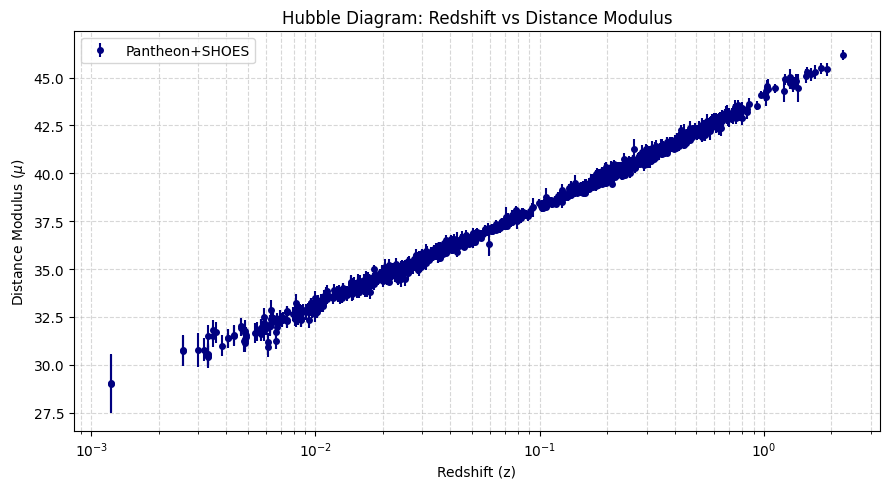
\includegraphics[width=0.78\textwidth]{hubble_diagram.png}
    \caption{Hubble diagram of Pantheon+SH0ES supernovae showing distance modulus $\mu$ versus redshift $z$. The monotonic rise reflects cosmic expansion and illustrates 
    the wide redshift coverage of the sample.}
    \label{fig:hubble_raw}
\end{figure}
\section{Methodology}
\subsection{Theoretical Framework}
Assuming flat $\Lambda$CDM, the Hubble parameter evolves as
\[
H(z) = H_0 \,\sqrt{\Omega_m(1+z)^3 + (1-\Omega_m)}.
\]
The luminosity distance and distance modulus are
\[
d_L(z) = (1+z)\frac{c}{H_0}\int_0^z \frac{dz'}{\sqrt{\Omega_m(1+z')^3 + (1-\Omega_m)}}, \qquad
\mu_{\mathrm{th}}(z) = 5\log_{10}\!\left(\frac{d_L(z)}{10\,\mathrm{pc}}\right).
\]

\subsection{Parameter Estimation}
We minimize
\[
\chi^2(H_0,\Omega_m) = \sum_i \frac{\big[\mu_{\mathrm{obs},i}-\mu_{\mathrm{th}}(z_i;H_0,\Omega_m)\big]^2}{\sigma_{\mu,i}^2}
\]
to obtain best-fit parameters and uncertainties (Gaussian approximation from the fit covariance). We also report a fixed-$\Omega_m$ variant and redshift-split consistency checks.

\subsection{Model Fit and Diagnostics}
\begin{figure}[H]
    \centering
    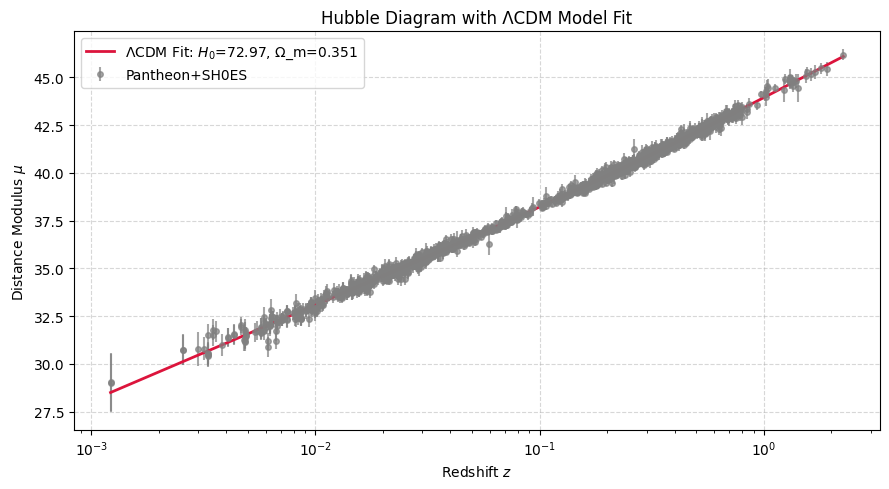
\includegraphics[width=0.78\textwidth]{cdm_fit.png}
    \caption{Hubble diagram with the best-fit flat $\Lambda$CDM model overlaid. Best-fit parameters: $H_0 \approx 72.97\ \mathrm{km\,s^{-1}\,Mpc^{-1}}$, $\Omega_m \approx 0.351$.}
    \label{fig:lcdm_fit}
\end{figure}

\begin{figure}[H]
    \centering
    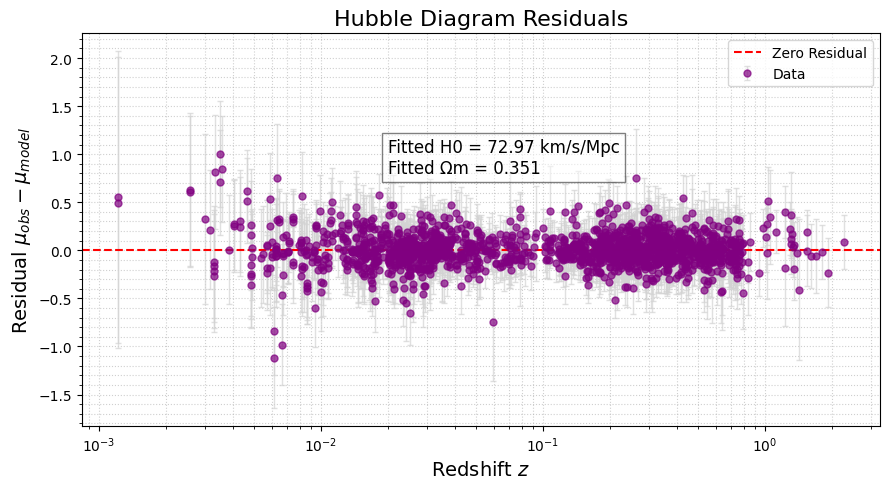
\includegraphics[width=0.78\textwidth]{hubble_residuals.png}
    \caption{Residuals $\Delta\mu=\mu_{\mathrm{obs}}-\mu_{\mathrm{th}}$ versus redshift. The scatter is centered near zero with no strong redshift trend.}
    \label{fig:resid_z}
\end{figure}

\begin{figure}[H]
    \centering
    \includegraphics[width=0.78\textwidth]{residuals_vs_distance_modulus.png}
    \caption{Residuals plotted against distance modulus. The absence of structure indicates no magnitude-dependent bias in the fit.}
    \label{fig:resid_mu}
\end{figure}

\begin{figure}[H]
    \centering
    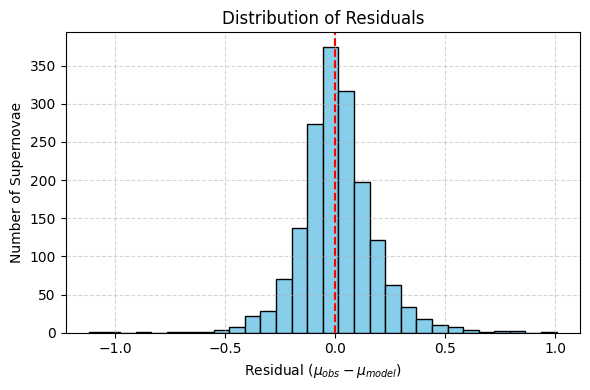
\includegraphics[width=0.6\textwidth]{residuals_histogram.png}
    \caption{Histogram of residuals. The distribution is centered near zero and approximately Gaussian, supporting the $\chi^2$ assumption.}
    \label{fig:resid_hist}
\end{figure}

\subsection{Age of the Universe}
With best-fit parameters, the age is computed via
\[
t_0 = \int_0^\infty \frac{dz}{(1+z)H(z)} \approx 12.36~\mathrm{Gyr}.
\]

\subsection{Implementation Notes}
Analysis used \texttt{pandas} for I/O, \texttt{Astropy} for cosmology helpers, \texttt{SciPy} for integration/optimization, and \texttt{Matplotlib} for visualization. 
Benign warnings were observed (a pandas \texttt{FutureWarning} for deprecated \texttt{delim\_whitespace}, a Matplotlib label \texttt{SyntaxWarning}, and a font glyph \texttt{UserWarning}); 
none affect numerical results.

\newpage
\section{Results and Discussion}
\subsection{Global Fits}
From the joint fit:
\[
H_0 = 72.97 \pm 0.26 \ \mathrm{km\,s^{-1}\,Mpc^{-1}}, \qquad \Omega_m = 0.351 \pm 0.019.
\]
Fixing $\Omega_m=0.3$ gives
\[
H_0 = 73.53 \pm 0.17 \ \mathrm{km\,s^{-1}\,Mpc^{-1}}.
\]
The derived age is $t_0 \approx 12.36$ Gyr.

\subsection{Implications}
Our $H_0$ agrees with the local SH0ES distance-ladder determination and remains in significant tension with the Planck 2018 CMB-inferred value. 
The higher $H_0$ naturally implies a younger universe than CMB-based $\Lambda$CDM ($\sim 13.8$ Gyr). The persistence of this discrepancy highlights 
the need for improved systematics control or extensions to the standard model.

\section{Limitations}
\subsection*{Dataset Constraints}
While the Pantheon+SH0ES catalog provides one of the most comprehensive compilations of Type~Ia supernovae to date, it is still subject to selection effects. 
Supernovae at higher redshifts suffer from reduced signal-to-noise, Malmquist bias, and calibration uncertainties in photometry. These factors can subtly bias 
distance moduli and hence inferred cosmological parameters.

\subsection*{Model Assumptions}
This study adopted the standard flat $\Lambda$CDM model. While this framework is widely successful, it assumes only matter and dark energy contributions with a 
constant equation of state $w=-1$. Potential extensions such as evolving dark energy, additional relativistic species, or spatial curvature were not considered here. 
If the Hubble tension reflects new physics, our restricted model space may underrepresent the true cosmology.

\subsection*{Parameter Degeneracies}
The analysis showed mild degeneracy between $H_0$ and $\Omega_m$, visible in the $\chi^2$ contour plot. Although the Pantheon+SH0ES data strongly constrain $H_0$, 
the degeneracy implies that joint fits with other cosmological probes (e.g., BAO, CMB) are necessary for breaking parameter correlations and improving robustness.

\subsection*{Systematic Uncertainties}
The accuracy of $H_0$ is limited not only by supernova photometry but also by calibration of the local distance ladder. While Pantheon+SH0ES incorporates 
Cepheid-calibrated anchors, 
alternative distance indicators (e.g., TRGB, strong-lensing time delays) sometimes yield discrepant results. Such systematics remain an open issue and could 
contribute to the persistent tension with Planck results.

\subsection*{Computational Limitations}
The implementation relied on numerical integration of the luminosity distance using \texttt{SciPy}. While sufficiently accurate for this analysis, more sophisticated treatments 
(e.g., Monte Carlo simulations of systematics, Bayesian hierarchical modeling) were not implemented due to time and computational constraints. These approaches could yield more precise uncertainty propagation.

\section{Conclusion}
In this study, we analyzed the Pantheon+SH0ES Type~Ia supernova dataset within the $\Lambda$CDM framework to obtain constraints on the Hubble constant and matter density parameter. 
The best-fit values,
\[
H_0 = 72.97 \pm 0.26 \ \mathrm{km\,s^{-1}\,Mpc^{-1}}, \qquad \Omega_m = 0.351 \pm 0.019,
\]
are consistent with recent local distance-ladder measurements but remain in significant tension with the CMB-based Planck result. The derived age of the Universe, $t_0 \approx 12.36 \ \mathrm{Gyr}$, 
further highlights the cosmological implications of this discrepancy.

Subsample analyses (low-$z$ vs.\ high-$z$) demonstrated robust consistency across redshift regimes, supporting the reliability of the Pantheon+SH0ES calibration. Additional tests with 
fixed $\Omega_m$ confirmed that the dataset tightly constrains the Hubble constant, independent of small variations in matter density.

The persistence of the Hubble tension underscores the importance of continued work in this area. Future progress will require both improved control of systematics in supernova cosmology and complementary 
constraints from alternative probes such as BAO, TRGB distances, and strong-lensing time delays. At the same time, the discrepancy may point toward physics beyond the standard $\Lambda$CDM model, 
including evolving dark energy or modifications to the early-Universe framework.

Overall, this project demonstrates the power of Type~Ia supernovae as precise cosmological probes and highlights their central role in one of the most pressing challenges of modern cosmology: 
reconciling the different routes to measuring the expansion rate of the Universe.

\newpage
\begin{thebibliography}{9}
\bibitem{Brout2022}
Brout, D., et al. (2022). The Pantheon+ Type Ia Supernova Catalog. \textit{The Astrophysical Journal}, 938(2), 110. \url{https://arxiv.org/abs/2202.04077}

\bibitem{Riess2022}
Riess, A. G., et al. (2022). A Comprehensive Measurement of the Local Value of the Hubble Constant with 1 km/s/Mpc Uncertainty from the Hubble Space Telescope and the SH0ES Team. 
\textit{The Astrophysical Journal Letters}, 934(1), L7. \url{https://arxiv.org/abs/2112.04510}

\bibitem{Planck2018}
Planck Collaboration. (2018). Planck 2018 results. VI. Cosmological parameters. \textit{Astronomy \& Astrophysics}, 641, A6. \url{https://arxiv.org/abs/1807.06209}

\bibitem{Astropy2013}
Astropy Collaboration. (2013). Astropy: A community Python package for astronomy. \textit{A\&A}, 558, A33. \url{https://arxiv.org/abs/1307.6212}

\bibitem{SciPy2020}
Virtanen, P., et al. (2020). SciPy 1.0: Fundamental Algorithms for Scientific Computing in Python. \textit{Nature Methods}, 17, 261--272. \url{https://doi.org/10.1038/s41592-019-0686-2}

\bibitem{Hubble1929}
Hubble, E. (1929). A relation between distance and radial velocity among extragalactic nebulae. \textit{PNAS}, 15(3), 168--173.

\bibitem{Ryden2017}
Ryden, B. (2017). \textit{Introduction to Cosmology} (2nd ed.). Cambridge University Press.
\end{thebibliography}
\newpage
\appendix
\section*{Appendix}
\subsection*{A. Additional Figure}

\begin{figure}[H]
    \centering
    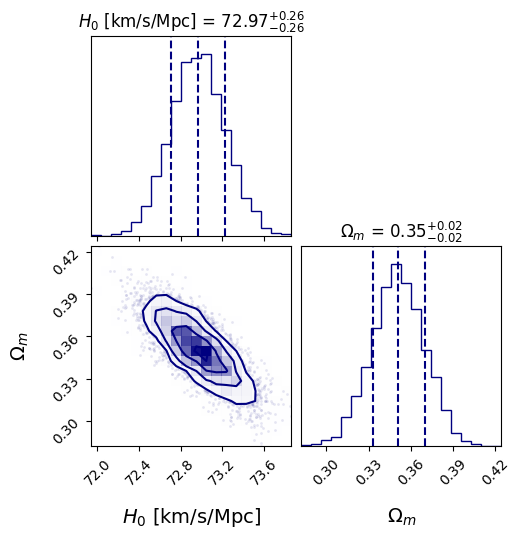
\includegraphics[width=0.7\textwidth]{corner.png}
    \caption{Joint posterior distribution of $H_0$ and $\Omega_m$. 
    The $1\sigma$ and $2\sigma$ confidence contours are indicated.}
\end{figure}
\subsection*{B. Supplementary Results}
\begin{table}[H]
    \centering
    \renewcommand{\arraystretch}{1.2} % spacing between rows
    \begin{tabular}{|l|c|}
        \hline
        \textbf{Parameter} & \textbf{Value} \\
        \hline
        Cosmological Model & Flat $\Lambda$CDM \\
        Best-fit $H_0$ & $72.97 \pm 0.26 \;\mathrm{km\,s^{-1}\,Mpc^{-1}}$ \\
        Best-fit $\Omega_m$ & $0.351 \pm 0.019$ \\
        Age of the Universe ($t_0$) & $12.36 \;\mathrm{Gyr}$ \\
        Fixed $\Omega_m$ Case & $\Omega_m = 0.30 \;\Rightarrow\; H_0 = 73.53 \pm 0.17 \;\mathrm{km\,s^{-1}\,Mpc^{-1}}$ \\
        Low-$z$ Subsample ($z<0.1$) & $H_0 = 73.01 \;\mathrm{km\,s^{-1}\,Mpc^{-1}}$ \\
        High-$z$ Subsample ($z\ge 0.1$) & $H_0 = 73.85 \;\mathrm{km\,s^{-1}\,Mpc^{-1}}$ \\
        \hline
    \end{tabular}
    \caption{Summary of key cosmological results from the Pantheon+SH0ES supernova analysis. Uncertainties are $1\sigma$.}
\end{table}
\end{document}